\chapter{Design and Implementation}
\label{chap:implementation}
Bla.

\section{Design and Implementation of the Context Broker}
\label{sec:broker}
This work first implements a regular Context Broker, with no fault tolerance resources. Then, it proposes a strategy to give the Broker High Availability function.
 
\subsection{Platform Choice}
The programming language chosen for the development of this work was Python. Python is a powerful and easy to learn modern programming language \cite{python}. It was chosen because it represents a challenge, and to show that the system is independent of the programmed language, i.e. different applications developed on different programming languages can interact with each other in the architecture, the messages exchanged are what matters. The Python IDE \cite{pycharm} was used, along with GitHub for version control \cite{github}.

The system was implemented over a HTTP REST (Representational State Transfer) Interface. A REST Interface is \cite{fielding2002principled}. For the RESTful implementation, Python Flask framework was used \cite{flask}.

For data persistence, MongoDB was used. MongoDB is a NoSQL 

\subsection{System Architecture}
In Figure \ref{fig:diagram} an overall diagram of the system is illustrated. Each node is a component of the system, and the arrows represent the interaction between them.

\begin{figure}[h]
	\centering
	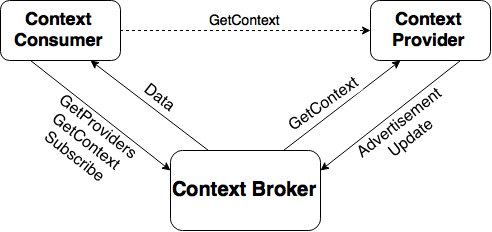
\includegraphics[scale=0.5]{diagram.png}
	\caption{Architecture diagram}
	\label{fig:diagram}
	
\end{figure}


\subsection{Broker Interfaces}
The Context Broker implements several interfaces for communication with the other system components. This section presents each interface and the way they were implemented: what they expect as input (HTTP request from Consumer or Provider), the action they perform, and what they provide as output (response to the Consumer or Provider).


\subsubsection{Advertisement}
\begin{itemize}
	\item[Input:] an Advertisement ContextML message, with Provider information
	
	\item[Action:] registers the Provider within the Broker
	
	\item[Output:] responds the Provider with a ACK or NACK ContextML message, informing success or error, with the corresponding error message.
\end{itemize}

\subsubsection{Update}
\begin{itemize}
	\item[Input:] a ctxEl ContextML Message, with context information to be registered in the Broker
	
	\item[Action:] registers in the Registry Table the context information, with its \textit{contextProvider}, \textit{scope} and \textit{entity} information, \textit{timestamp} and expiration date (\textit{expires}) of the information. It also checks if a \textbf{Subscription} exists for the updated information, sending it to the Consumer \textit{callbackUrl}, when applied.
	
	\item[Output:] responds the Provider with a ACK or NACK ContextML message, informing success or error, with the corresponding error message.
\end{itemize}

\subsubsection{Get Providers}
\begin{itemize}
	\item[Input:] \textit{scope} (mandatory) and \textit{entity type} (optional) arguments in the URL
	
	\item[Action:] looks for registered Providers that provide information matching the arguments given
	
	\item[Output:] responds the Consumer with Providers Lookup ContextML message, containing a list of the providers that match the requested arguments
\end{itemize}

\subsubsection{Get Context}
\begin{itemize}
	\item[Input:] from the Consumer, arguments \textit{scope} and \textit{entity} in the URL
	
	\item[Action:] looks for the latest Context information in the registry that matches the entity and scope received
	
	\item[Output:] responds the Consumer with a ctxEls ContextML message, containing the , or with a NACK ContextML message, informing the error.
	
\end{itemize}
* As seen in Figure \ref{fig:diagram}, there can also exist a direct \textit{GetContext} request from the Consumer to the Provider, thus not involving the Broker. This can be done by the Consumer asking the Broker for a providers list regarding a certain \textit{scope}, and then asking it directly for the desired context information. 

\subsubsection{Subscribe}
\begin{itemize}
	\item[Input:] arguments as follows:  \textit{callbackUrl}, with the URL to where the Broker sends the content it is subscribed to; \textit{scope} and \textit{entity}, with corresponding information the consumer wants to subscribe to; and \textit{minutes}, with the amount of time, in minutes, that the subscription is valid.
	
	\item[Action:] registers the subscription
	
	\item[Output:] responds the Provider with a ACK or NACK ContextML message, informing success or error, with the corresponding error message.
\end{itemize}

\section{Introducing High Availability Technique}
\label{sec:ha_broker}

\subsection{Objective}

\subsection{Design}

\subsection{Protocol created}
Using \cite{protobuf}